\documentclass[DM,authoryear,toc]{lsstdoc}
\input{meta}

% Package imports go here.

% Local commands go here.

%If you want glossaries
%\input{aglossary.tex}
%\makeglossaries

\title{Real-bogus classifier -- status report}

% Optional subtitle
% \setDocSubtitle{A subtitle}

\author{%
Nima Sedaghat
}

\setDocRef{DMTN-272}
\setDocUpstreamLocation{\url{https://github.com/lsst-dm/dmtn-272}}

\date{\vcsDate}

% Optional: name of the document's curator
% \setDocCurator{The Curator of this Document}

\setDocAbstract{%
We report the current status of the real-bogus classifier. The report starts with the design and technical aspects and continues to show quantitative and qualitative evaluations.
}

% Change history defined here.
% Order: oldest first.
% Fields: VERSION, DATE, DESCRIPTION, OWNER NAME.
% See LPM-51 for version number policy.
\setDocChangeRecord{%
  \addtohist{1}{YYYY-MM-DD}{Unreleased.}{Nima Sedaghat}
}

\usepackage{grffile}

\begin{document}

% Create the title page.
\maketitle
% Frequently for a technote we do not want a title page  uncomment this to remove the title page and changelog.
% use \mkshorttitle to remove the extra pages

% ADD CONTENT HERE
% You can also use the \input command to include several content files.

\section{Architecture}
So far, we have run the experiments with three different architectures:

\begin{itemize}
\item{An off-the-shelf architecture based on ResNet50~\citep{he2016deep}.}
\item{An off-the-shelf architecture based on VGG6~\citep{simonyan2014very}.}
\item{A custom architecture based on the encoder part of TransiNet, internally referred to as rbTN~\citep{sedaghat2018effective}.}
\end{itemize}

The former two (ResNet50 and VGG6) have been more extensively tested.

\section{Data}
We used the version of the DC2 dataset available as a butler repository, as the main source of our data.

We have chosen the tract 3080 for training and 4024 for test/validation. Reasoning TBA.
Figures~\ref{fig:exposure_hist}~,~\ref{fig:detector_hist} show the distributions of exposure ($\sim$visit) and detector numbers in the raw images currently captured (simulated) in each ot the chosen tracts. The detector indices are, neglecting the narrow peaks, roughly uniformly distributed, meaning that we have an almost equal number of raw images (roughly 300) for each detector/CCD in each of the chosen tracts. This is particularly important for the training phase as we do not want the model to be biased towards specific detector characteristics.

More details about the exact data-set used for each experiment is included in the experiment's subsection.

\begin{figure}[h!]
  \centering
  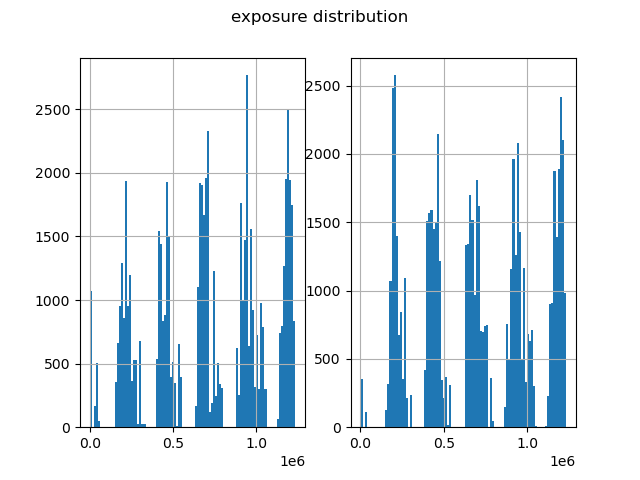
\includegraphics[width=0.7\textwidth]{exposure_hist.png}
  \caption{Distribution of exposure numbers of the existing raw images of each of the tracts. Left: tract \#3080, right: tract \#4024.}
  \label{fig:exposure_hist}
\end{figure}

\begin{figure}[h!]
  \centering
  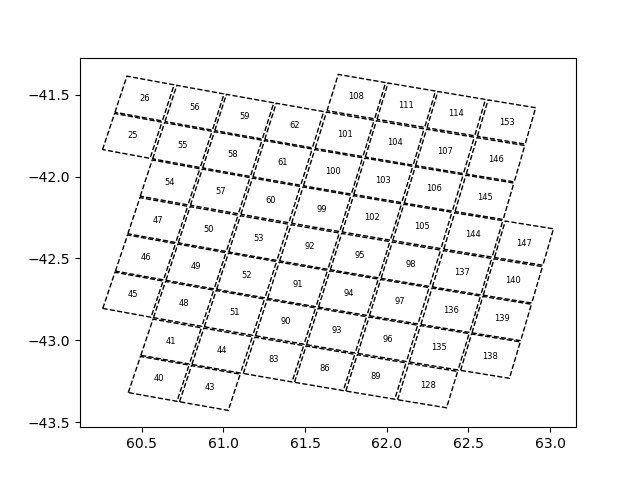
\includegraphics[width=0.7\textwidth]{tract_detectors.png}
  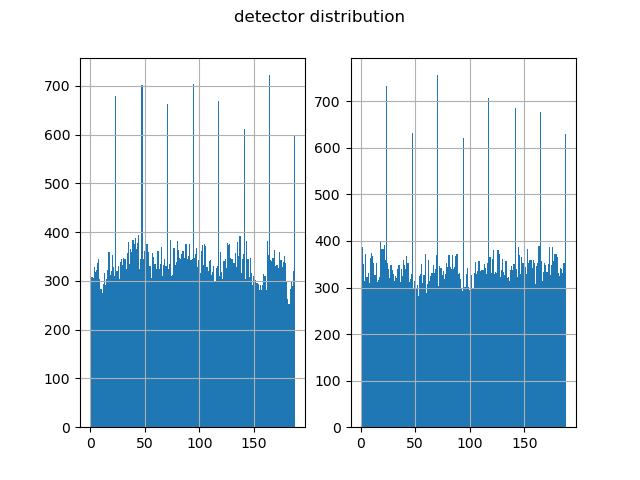
\includegraphics[width=0.7\textwidth]{detector_hist.png}
  \caption{On the top, the detectors (CCD) are illustrated with their relative spatial arrangement. The bottom two images depict the distribution of detector indices of the existing raw images of each of the tracts. Left: tract \#3080, right: tract \#4024.}
  \label{fig:detector_hist}
\end{figure}

\clearpage
Template images were created per-tract, in the sense that the data input to the APTemplate pipeline was constrained to a single tract at each run. Figure~\ref{fig:tract_templates} illustrates an exemplar instance, where the effect of limiting the raws to a single tract apperas as croppings in the output templates. This is not of a concern in this very application though, since the downstream tasks receive proper masks and will generate cutouts only of the regions from which enough informative data can be extracted.

\begin{figure}[h]
  \centering
  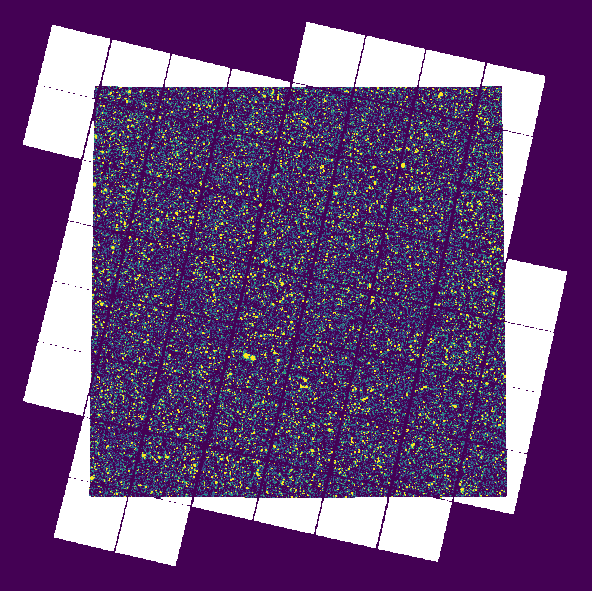
\includegraphics[width=0.7\textwidth]{tract_templates.png}
  \caption{Templates generated based on raw images from a single tract. The white chessboard in the background is the spatial spread of the detectors (a single visit/exposure), whereas the area ``full of stars'' represents a single tract in the sky.}
  \label{fig:tract_templates}
\end{figure}

%----------------------------------------------------
\clearpage
\section{Evaluation Results}

\subsection{The ``PCW 2022'' network and data}
The data-set used for training this model, DL Dataset v0.1.1, consists of \texttt{78222} triplets, out of which \texttt{2591} triplets ($\sim 3\%$) are \texttt{positive}s.

\begin{figure}[h]
  \centering
  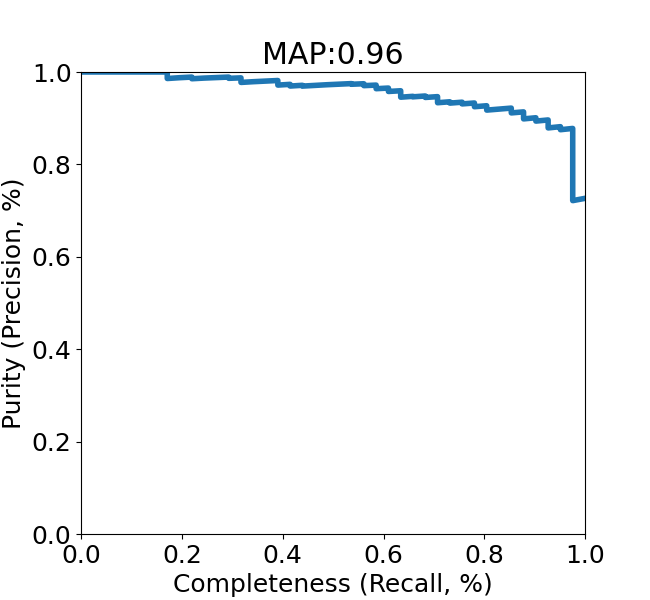
\includegraphics[width=0.5\textwidth]{precrec___checkpoint_epoch0000087_0200000____rbdata_data_npy_data_gt1M___posw_30.png}
  \caption{No sigma-thresholding applied on the input sources (diffim output)}
  \label{fig:tract_templates}
\end{figure}

\begin{figure}[h]
  \centering
  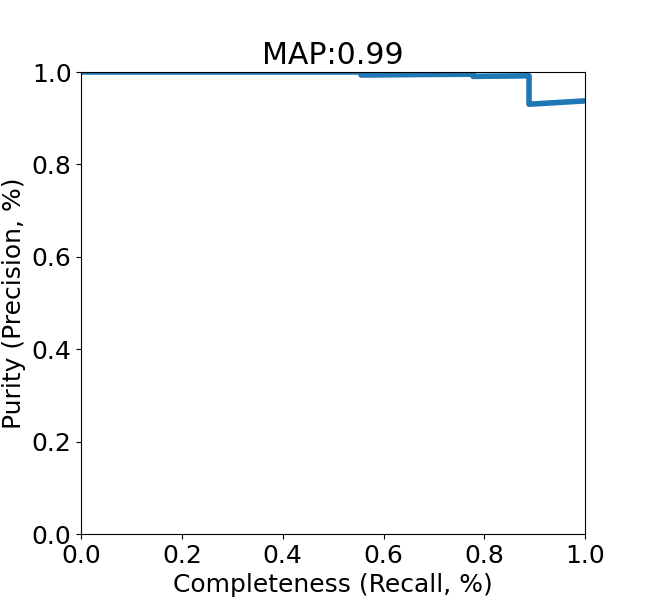
\includegraphics[width=0.5\textwidth]{precrec___checkpoint_epoch0000087_0200000____rbdata_data_npy_data_gt1M-5sigma___posw_30.png}
  \caption{Only sources with $snr > 5\sigma$}
  \label{fig:tract_templates}
\end{figure}

\begin{figure}[h]
  \centering
  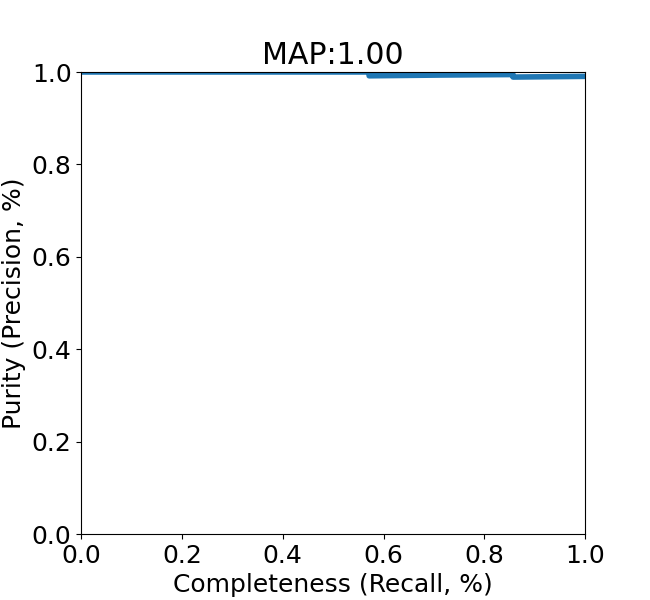
\includegraphics[width=0.5\textwidth]{precrec___checkpoint_epoch0000087_0200000____rbdata_data_npy_data_gt1M-6sigma___posw_30.png}
  \caption{Only sources with $snr > 6\sigma$}
  \label{fig:tract_templates}
\end{figure}

% ----------------------------------------------------
\clearpage
\subsection{New Dataset}
The new dataset (DL v0.1.2) is essentially the same as the previous version (v.0.1.1), only regenerated with a more recent version of the stack (\texttt{w\_2023\_38}). The number of images is relatively higher though, in the new version: there are \texttt{183750} triplets, out of which \texttt{10147} ($\sim 5\%$) are positives.

We used a $95-5$ training-validation split, which leaves us with \texttt{9198} validation triplets (with \texttt{533} $\simeq 5\%$ positives).


\begin{figure}[h]
  \centering
  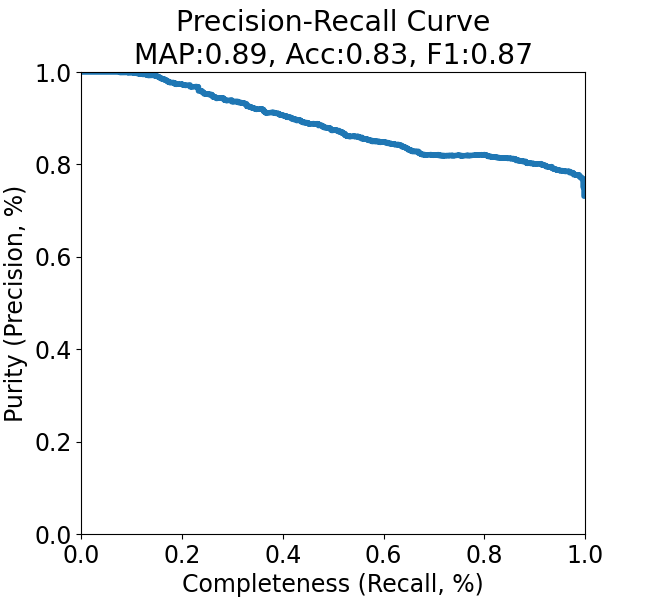
\includegraphics[width=0.4\textwidth]{precrec_13-resnet50-FullAugmentation-scratch-B64__0255000__npy_data_0.1.2-0sigma_256by256__posw_20.png}
  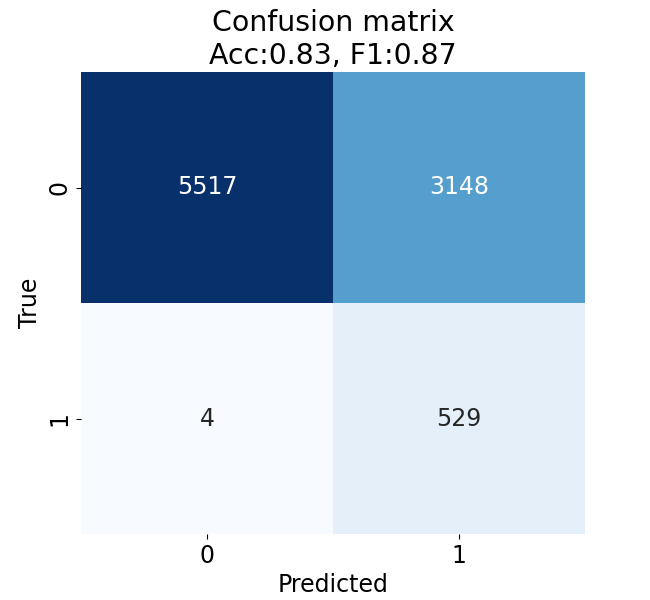
\includegraphics[width=0.4\textwidth]{confmat_13-resnet50-FullAugmentation-scratch-B64__0255000__npy_data_0.1.2-0sigma_256by256__posw_20.png}
  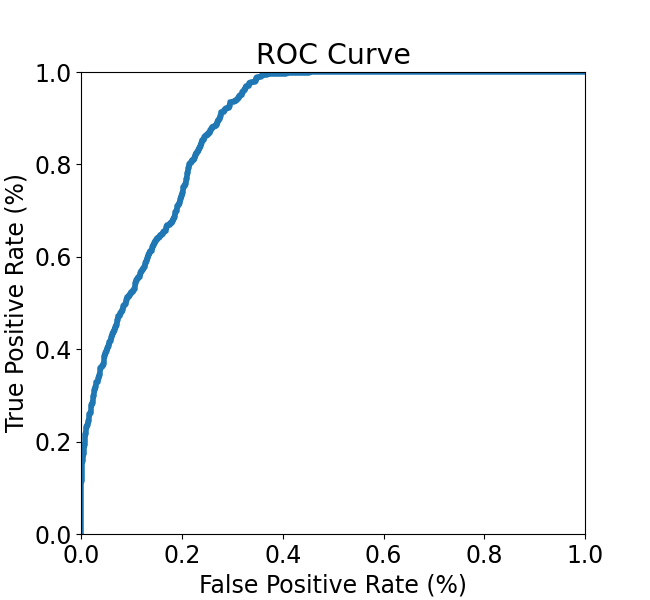
\includegraphics[width=0.4\textwidth]{roc_13-resnet50-FullAugmentation-scratch-B64__0255000__npy_data_0.1.2-0sigma_256by256__posw_20.png}
  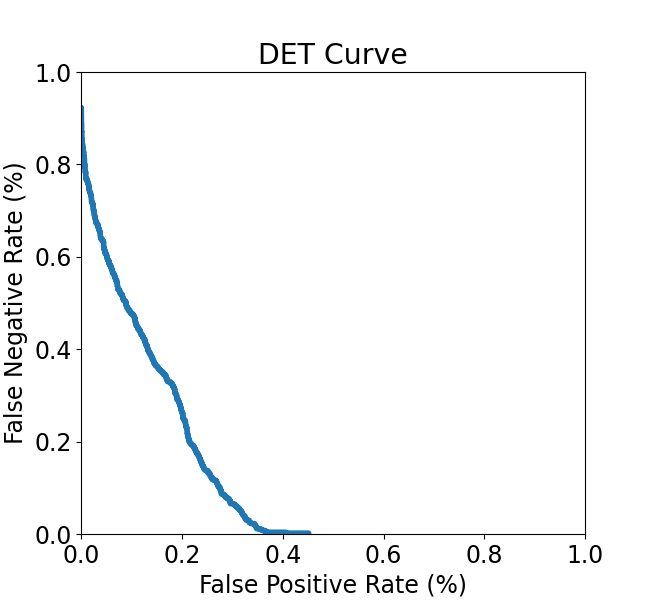
\includegraphics[width=0.4\textwidth]{det_13-resnet50-FullAugmentation-scratch-B64__0255000__npy_data_0.1.2-0sigma_256by256__posw_20.png}
  \caption{Evaluation results based on the whole dataset.}
  \label{fig:tract_templates}
\end{figure}

\begin{figure}[h]
  \centering
  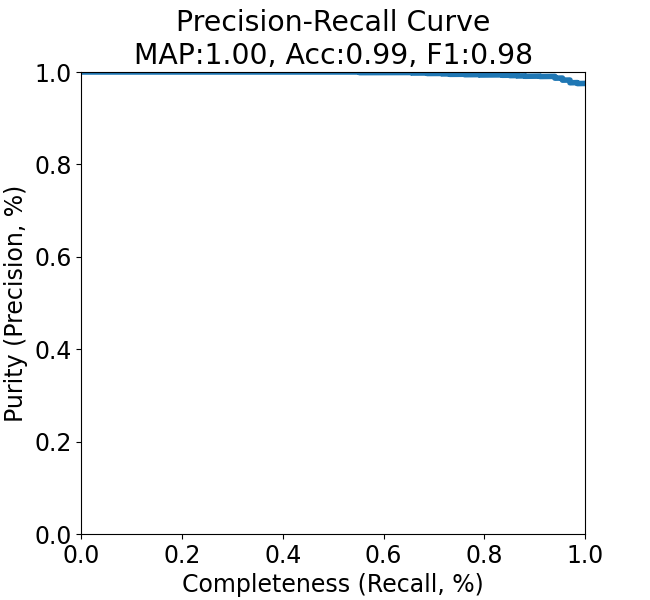
\includegraphics[width=0.4\textwidth]{precrec_13-resnet50-FullAugmentation-scratch-B64__0255000__npy_data_0.1.2-5sigma_256by256__posw_20.png}
  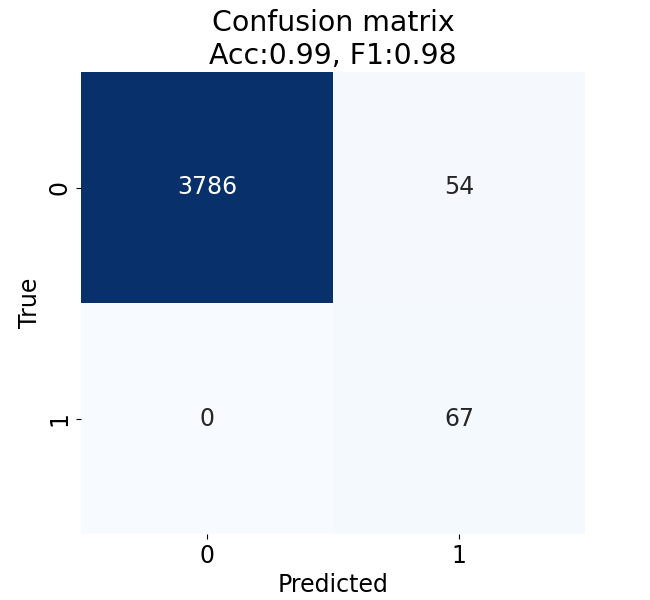
\includegraphics[width=0.4\textwidth]{confmat_13-resnet50-FullAugmentation-scratch-B64__0255000__npy_data_0.1.2-5sigma_256by256__posw_20.png}
  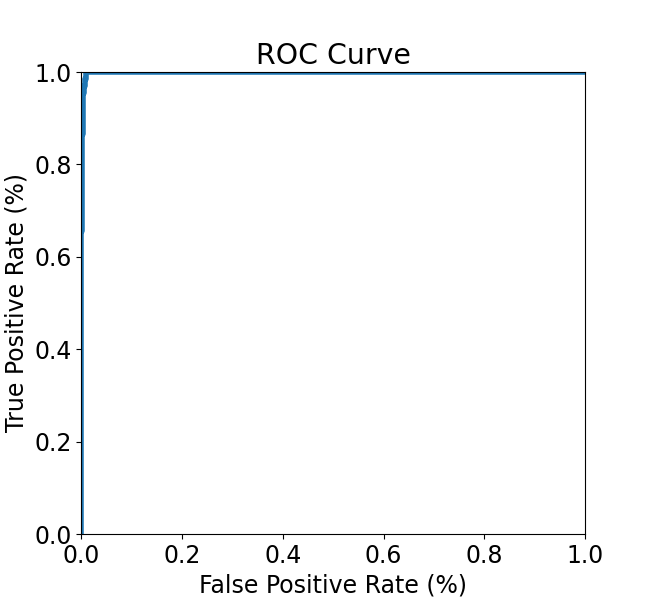
\includegraphics[width=0.4\textwidth]{roc_13-resnet50-FullAugmentation-scratch-B64__0255000__npy_data_0.1.2-5sigma_256by256__posw_20.png}
  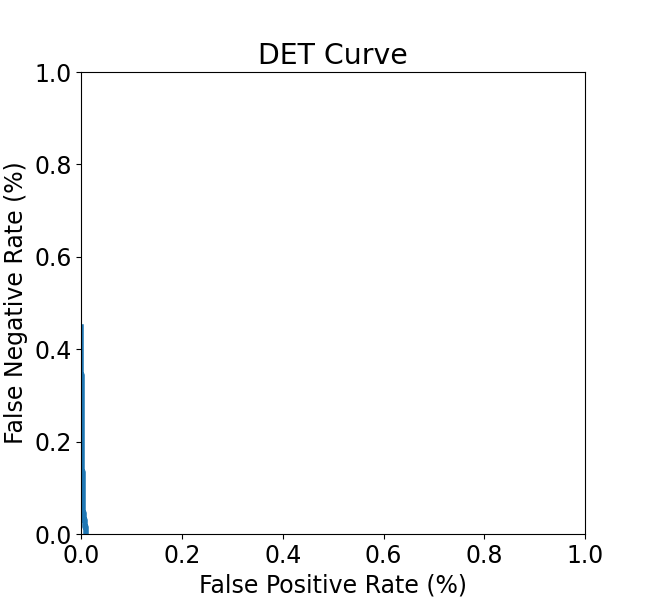
\includegraphics[width=0.4\textwidth]{det_13-resnet50-FullAugmentation-scratch-B64__0255000__npy_data_0.1.2-5sigma_256by256__posw_20.png}
  \caption{Only sources with $snr > 5\sigma$}
  \label{fig:tract_templates}
\end{figure}

\begin{figure}[h]
  \centering
  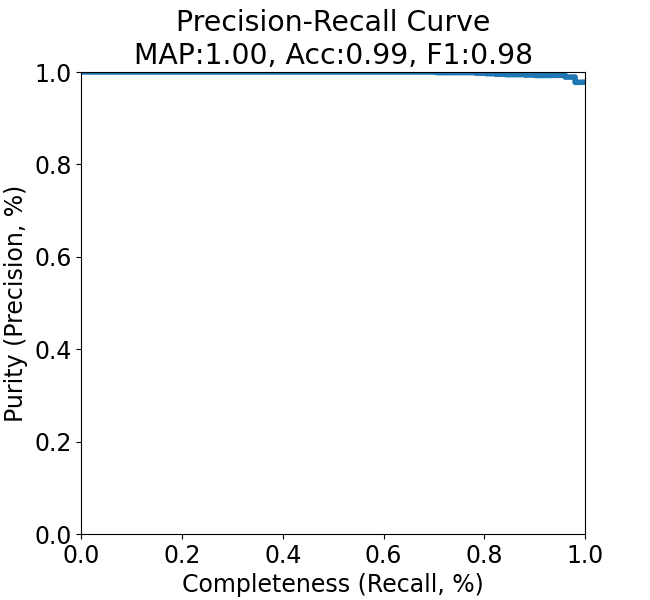
\includegraphics[width=0.4\textwidth]{precrec_13-resnet50-FullAugmentation-scratch-B64__0255000__npy_data_0.1.2-6sigma_256by256__posw_20.png}
  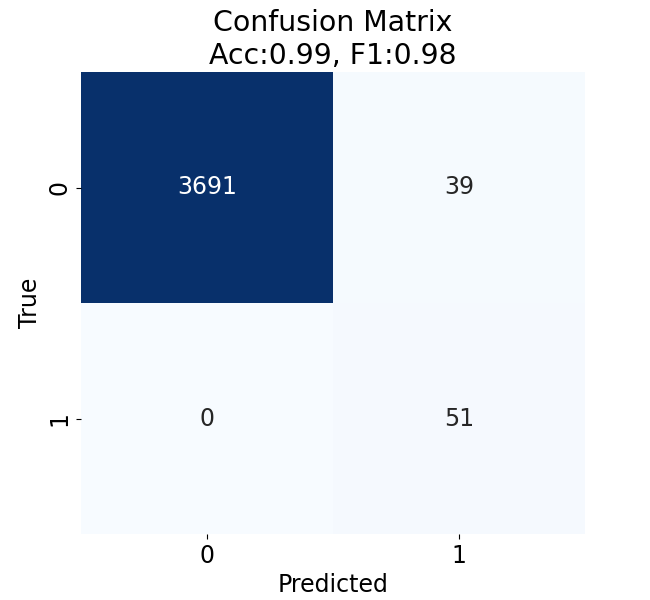
\includegraphics[width=0.4\textwidth]{confmat_13-resnet50-FullAugmentation-scratch-B64__0255000__npy_data_0.1.2-6sigma_256by256__posw_20.png}
  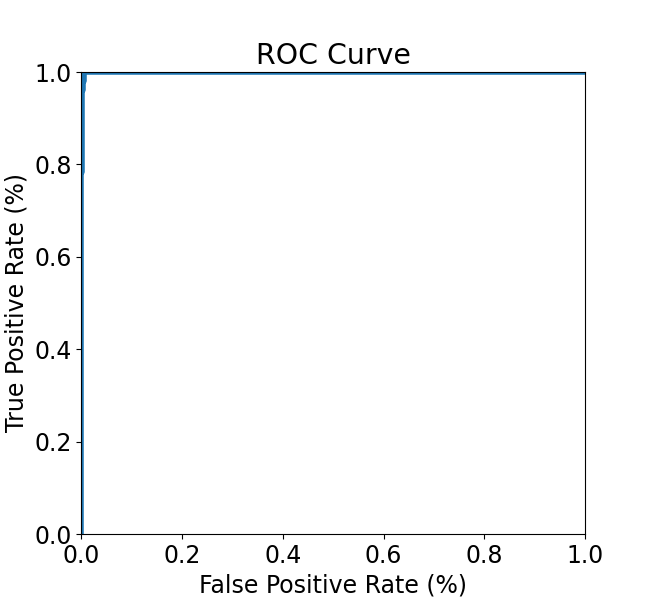
\includegraphics[width=0.4\textwidth]{roc_13-resnet50-FullAugmentation-scratch-B64__0255000__npy_data_0.1.2-6sigma_256by256__posw_20.png}
  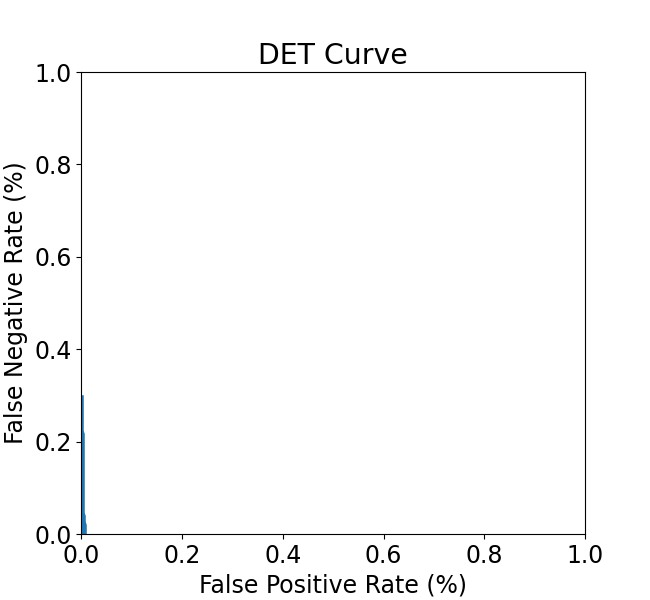
\includegraphics[width=0.4\textwidth]{det_13-resnet50-FullAugmentation-scratch-B64__0255000__npy_data_0.1.2-6sigma_256by256__posw_20.png}
  \caption{Only sources with $snr > 6\sigma$}
  \label{fig:tract_templates}
\end{figure}

\clearpage

\subsection{New Dataset -- No Weight Balancing}

\begin{figure}[h]
  \centering
  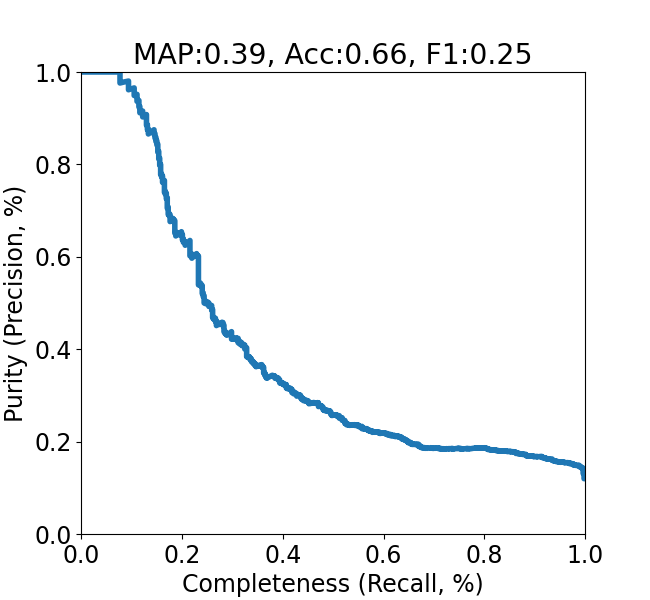
\includegraphics[width=0.4\textwidth]{precrec_13-resnet50-FullAugmentation-scratch-B64__0255000__npy_data_0.1.2-0sigma_256by256__posw_1.png}
  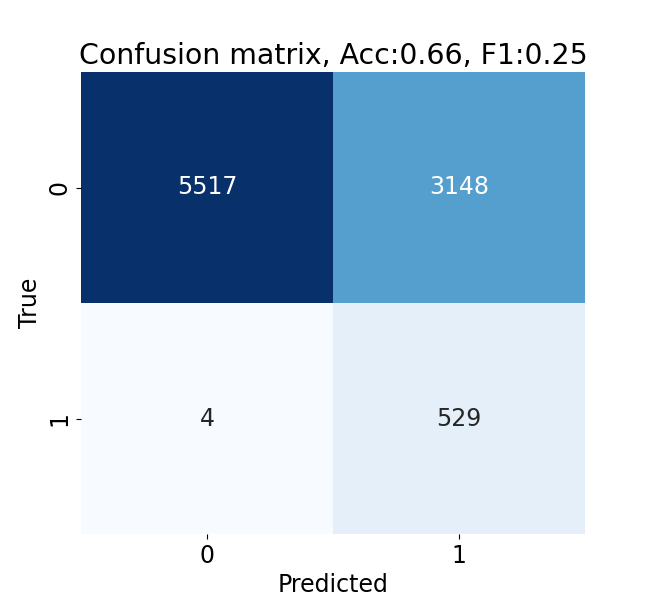
\includegraphics[width=0.4\textwidth]{confmat_13-resnet50-FullAugmentation-scratch-B64__0255000__npy_data_0.1.2-0sigma_256by256__posw_1.png}
  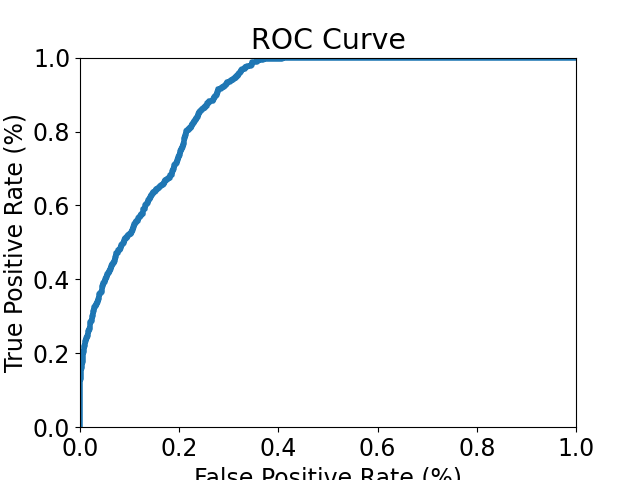
\includegraphics[width=0.4\textwidth]{roc_13-resnet50-FullAugmentation-scratch-B64__0255000__npy_data_0.1.2-0sigma_256by256__posw_1.png}
  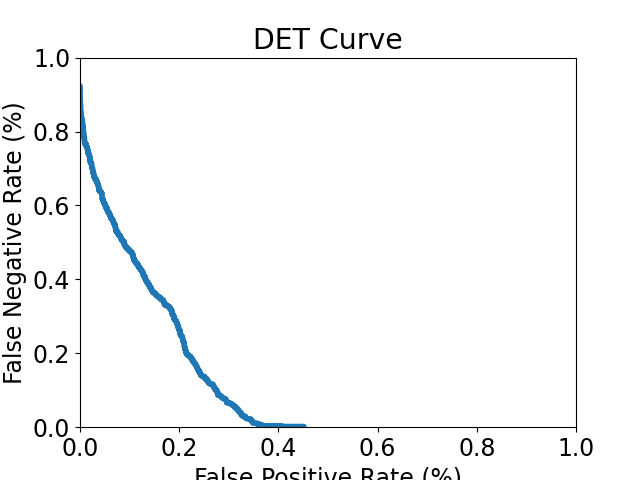
\includegraphics[width=0.4\textwidth]{det_13-resnet50-FullAugmentation-scratch-B64__0255000__npy_data_0.1.2-0sigma_256by256__posw_1.png}
  \caption{Evaluation results based on the whole dataset.}
  \label{fig:tract_templates}
\end{figure}

\begin{figure}[h]
  \centering
  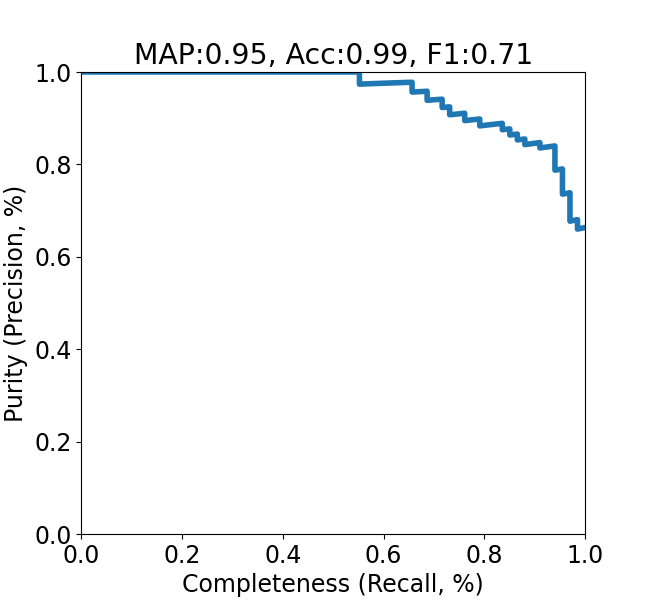
\includegraphics[width=0.4\textwidth]{precrec_13-resnet50-FullAugmentation-scratch-B64__0255000__npy_data_0.1.2-5sigma_256by256__posw_1.png}
  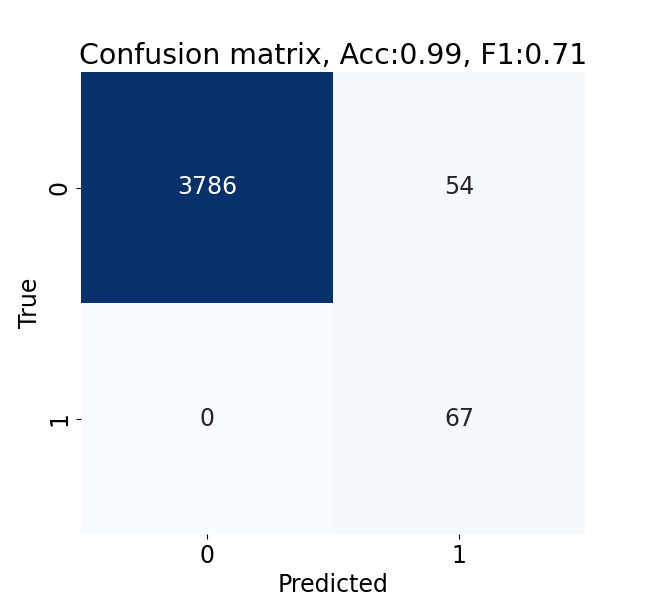
\includegraphics[width=0.4\textwidth]{confmat_13-resnet50-FullAugmentation-scratch-B64__0255000__npy_data_0.1.2-5sigma_256by256__posw_1.png}
  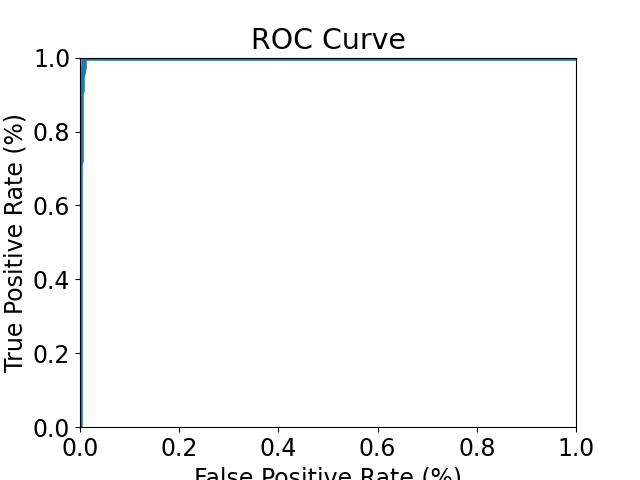
\includegraphics[width=0.4\textwidth]{roc_13-resnet50-FullAugmentation-scratch-B64__0255000__npy_data_0.1.2-5sigma_256by256__posw_1.png}
  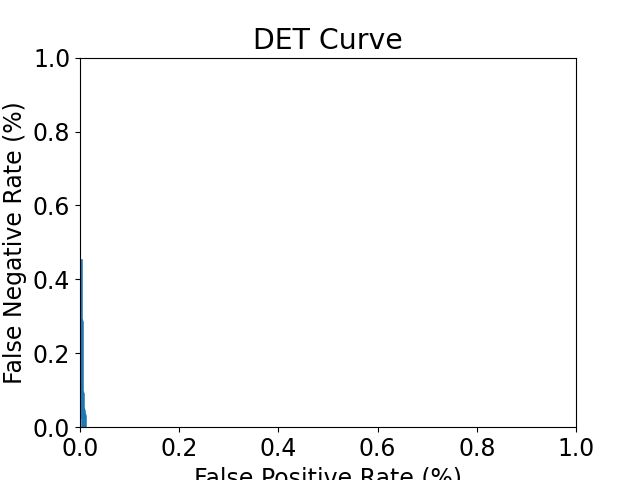
\includegraphics[width=0.4\textwidth]{det_13-resnet50-FullAugmentation-scratch-B64__0255000__npy_data_0.1.2-5sigma_256by256__posw_1.png}
  \caption{Only sources with $snr > 5\sigma$}
  \label{fig:tract_templates}
\end{figure}

\begin{figure}[h]
  \centering
  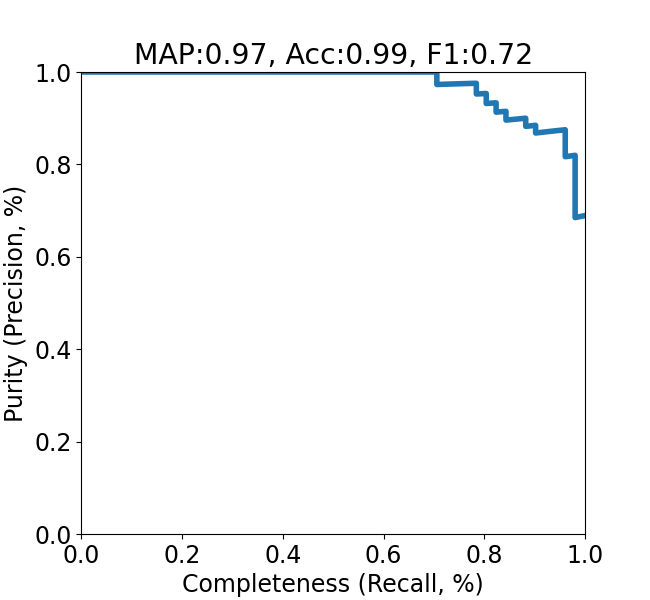
\includegraphics[width=0.4\textwidth]{precrec_13-resnet50-FullAugmentation-scratch-B64__0255000__npy_data_0.1.2-6sigma_256by256__posw_1.png}
  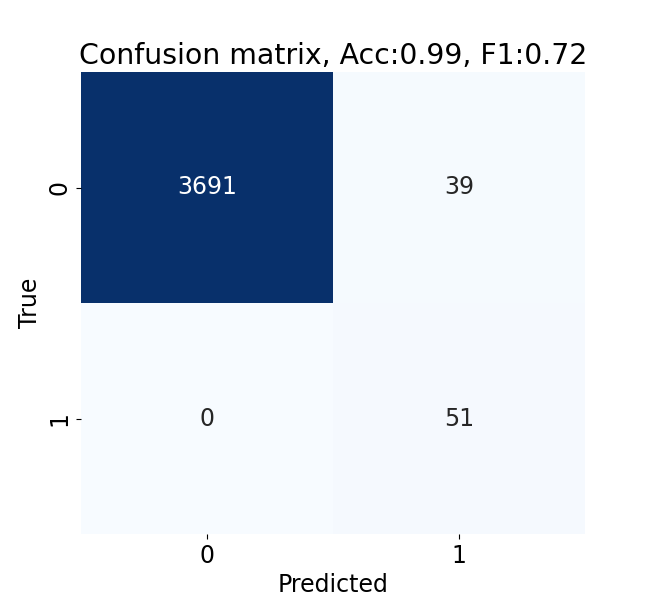
\includegraphics[width=0.4\textwidth]{confmat_13-resnet50-FullAugmentation-scratch-B64__0255000__npy_data_0.1.2-6sigma_256by256__posw_1.png}
  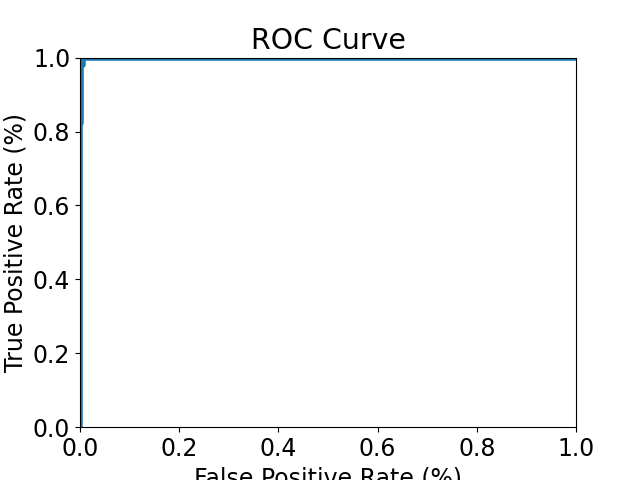
\includegraphics[width=0.4\textwidth]{roc_13-resnet50-FullAugmentation-scratch-B64__0255000__npy_data_0.1.2-6sigma_256by256__posw_1.png}
  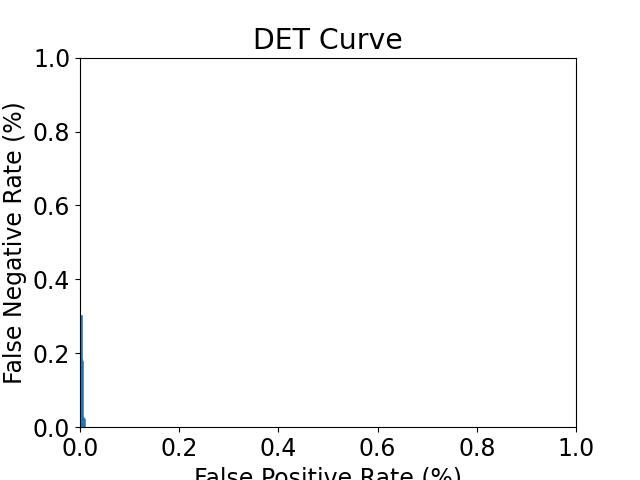
\includegraphics[width=0.4\textwidth]{det_13-resnet50-FullAugmentation-scratch-B64__0255000__npy_data_0.1.2-6sigma_256by256__posw_1.png}
  \caption{Only sources with $snr > 6\sigma$}
  \label{fig:tract_templates}
\end{figure}

\clearpage


\appendix
% Include all the relevant bib files.
% https://lsst-texmf.lsst.io/lsstdoc.html#bibliographies
\section{References} \label{sec:bib}
\renewcommand{\refname}{} % Suppress default Bibliography section
\bibliography{local,lsst,lsst-dm,refs_ads,refs,books}

% Make sure lsst-texmf/bin/generateAcronyms.py is in your path
\section{Acronyms} \label{sec:acronyms}
\addtocounter{table}{-1}
\begin{longtable}{p{0.145\textwidth}p{0.8\textwidth}}\hline
\textbf{Acronym} & \textbf{Description}  \\\hline

DM & Data Management \\\hline
DMTN & DM Technical Note \\\hline
\end{longtable}

% If you want glossary uncomment below -- comment out the two lines above
%\printglossaries





\end{document}
